\documentclass[12pt,a4paper]{article}
\usepackage[utf8]{inputenc}
\usepackage{amsmath,amssymb,amsfonts}
\usepackage{graphicx}
\usepackage{tikz}
\usepackage{pgfplots}
\usepackage{float}
\usepackage{array}
\usepackage{booktabs}
\usepackage{enumitem}
\usepackage{caption}
\usepackage{subcaption}
\usepackage{geometry}
\pgfplotsset{compat=newest}

\geometry{margin=2.5cm}

\title{Soal Latihan Riset Operasi}
\author{Rifqi Fadil Fahrial - 1222646}
\date{}

\begin{document}

\maketitle

\begin{enumerate}
    \item \textbf{Soal 1: Masalah Optimasi Produksi Mebel}
    
    Suatu perusahaan mebel memerlukan 18 unsur A dan 24 unsur B per hari. Untuk membuat barang jenis I dibutuhkan 1 unsur A dan 2 unsur B, sedangkan untuk membuat barang jenis II dibutuhkan 3 unsur A dan 2 unsur B. Jika barang jenis I dijual seharga Rp 250.000,00 per unit dan barang jenis II dijual seharga Rp 400.000,00 per unit, maka agar penjualannya mencapai maksimum, berapa banyak masing-masing barang harus dibuat?
    
    \textbf{Penyelesaian dengan Metode Grafik:}
    
    Langkah 1: Menentukan variabel keputusan
    \begin{align*}
    x_1 &= \text{jumlah barang jenis I yang diproduksi per hari} \\
    x_2 &= \text{jumlah barang jenis II yang diproduksi per hari}
    \end{align*}
    
    Langkah 2: Menentukan fungsi tujuan
    
    Fungsi tujuan adalah memaksimalkan keuntungan penjualan:
    \begin{align*}
    Z &= 250.000x_1 + 400.000x_2
    \end{align*}
    
    Langkah 3: Menentukan kendala-kendala
    \begin{align*}
    \text{Kendala unsur A:} \quad 1x_1 + 3x_2 &\leq 18 \\
    \text{Kendala unsur B:} \quad 2x_1 + 2x_2 &\leq 24 \\
    \text{Non-negatif:} \quad x_1, x_2 &\geq 0
    \end{align*}
    
    Langkah 4: Menggambar kendala-kendala
    
    a) Untuk kendala $1x_1 + 3x_2 \leq 18$, kita cari titik-titik potong dengan sumbu:
    \begin{align*}
    \text{Jika } x_1 = 0 &\Rightarrow 3x_2 = 18 \Rightarrow x_2 = 6 \text{ (titik potong di } (0,6)) \\
    \text{Jika } x_2 = 0 &\Rightarrow x_1 = 18 \text{ (titik potong di } (18,0))
    \end{align*}
    
    b) Untuk kendala $2x_1 + 2x_2 \leq 24$, kita sederhanakan menjadi $x_1 + x_2 \leq 12$:
    \begin{align*}
    \text{Jika } x_1 = 0 &\Rightarrow x_2 = 12 \text{ (titik potong di } (0,12)) \\
    \text{Jika } x_2 = 0 &\Rightarrow x_1 = 12 \text{ (titik potong di } (12,0))
    \end{align*}
    
    \begin{figure}[H]
    \centering
    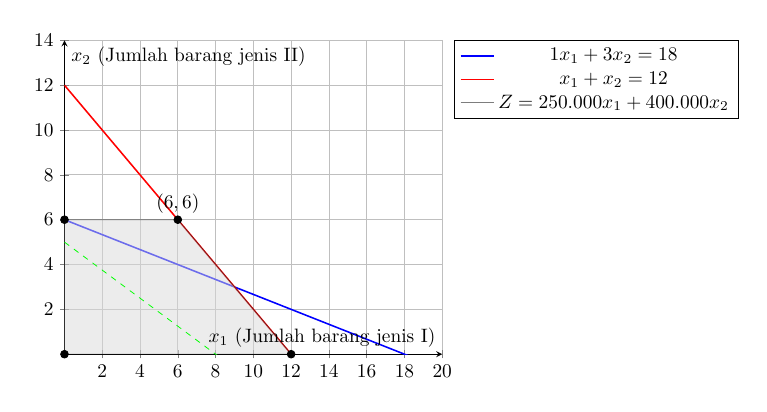
\begin{tikzpicture}[scale=0.7]
    \begin{axis}[
        axis lines=middle,
        grid=both,
        xmin=0, xmax=20,
        ymin=0, ymax=14,
        xtick={0,2,...,20},
        ytick={0,2,...,14},
        xlabel={$x_1$ (Jumlah barang jenis I)},
        ylabel={$x_2$ (Jumlah barang jenis II)},
        legend pos=outer north east
    ]
    
    % Kendala unsur A: 1x₁ + 3x₂ ≤ 18
    \addplot[domain=0:20, thick, blue] {(18-x)/3};
    \addlegendentry{$1x_1 + 3x_2 = 18$}
    
    % Kendala unsur B: 2x₁ + 2x₂ ≤ 24 atau x₁ + x₂ ≤ 12
    \addplot[domain=0:20, thick, red] {12-x};
    \addlegendentry{$x_1 + x_2 = 12$}
    
    % Daerah fisibel
    \addplot[fill=gray!30, opacity=0.5] coordinates {
        (0,0) (0,6) (6,6) (12,0) (0,0)
    } \closedcycle;
    
    % Titik-titik sudut
    \addplot[mark=*, color=black] coordinates {(0,0)} node[anchor=north east] {$(0,0)$};
    \addplot[mark=*, color=black] coordinates {(0,6)} node[anchor=south east] {$(0,6)$};
    \addplot[mark=*, color=black] coordinates {(6,6)} node[anchor=south] {$(6,6)$};
    \addplot[mark=*, color=black] coordinates {(12,0)} node[anchor=north west] {$(12,0)$};
    
    % Garis fungsi tujuan
    \addplot[domain=0:20, dashed, green] {(5-0.625*x)};
    \addlegendentry{$Z = 250.000x_1 + 400.000x_2$}
    
    \end{axis}
    \end{tikzpicture}
    \caption{Daerah Fisibel dan Titik Optimal - Masalah Produksi Mebel}
    \end{figure}
    
    Langkah 5: Menentukan titik-titik sudut daerah fisibel:
    \begin{align*}
    &(0,0) && \text{titik asal} \\
    &(0,6) && \text{titik potong kendala 1 dengan sumbu } x_2 \\
    &(6,6) && \text{titik potong kendala 1 dan kendala 2} \\
    &(12,0) && \text{titik potong kendala 2 dengan sumbu } x_1
    \end{align*}
    
    Titik $(6,6)$ diperoleh dari penyelesaian sistem persamaan:
    \begin{align*}
    1x_1 + 3x_2 &= 18 \quad \ldots (1) \\
    x_1 + x_2 &= 12 \quad \ldots (2)
    \end{align*}
    
    Dari persamaan (2): $x_1 = 12 - x_2$
    
    Substitusi ke persamaan (1):
    \begin{align*}
    1(12 - x_2) + 3x_2 &= 18 \\
    12 - x_2 + 3x_2 &= 18 \\
    12 + 2x_2 &= 18 \\
    2x_2 &= 6 \\
    x_2 &= 3
    \end{align*}
    
    Kemudian $x_1 = 12 - x_2 = 12 - 3 = 9$
    
    Jadi titik potongnya adalah $(9,3)$.
    
    Langkah 6: Mengevaluasi fungsi tujuan di setiap titik sudut:
    \begin{align*}
    Z(0,0) &= 250.000(0) + 400.000(0) = 0 \\
    Z(0,6) &= 250.000(0) + 400.000(6) = 2.400.000 \\
    Z(9,3) &= 250.000(9) + 400.000(3) = 2.250.000 + 1.200.000 = 3.450.000 \\
    Z(12,0) &= 250.000(12) + 400.000(0) = 3.000.000
    \end{align*}
    
    Nilai maksimum fungsi tujuan tercapai pada titik $(9,3)$ dengan nilai $Z = 3.450.000$.
    
    Jadi, agar penjualan mencapai maksimum, perusahaan harus memproduksi 9 unit barang jenis I dan 3 unit barang jenis II per hari, dengan total keuntungan sebesar Rp 3.450.000,00.
    
    \item \textbf{Soal 2: Masalah Optimasi Produksi PT Yummy Food}
    
    PT Yummy food memiliki sebuah pabrik yang akan memproduksi dua jenis produk yaitu vanilla dan violette. Untuk memproduksi kedua produk tersebut diperlukan bahan baku A, bahan baku B, dan tenaga kerja. Maksimum pengerjaan bahan baku A adalah 60kg per hari, bahan baku B 30kg per hari dan tenaga kerja 40jam per hari. Kedua jenis produk memberikan sumbangan keuntungan sebesar Rp40,00 untuk vanilla dan Rp30,00 untuk violette. Masalah yang dihadapi adalah bagaimana menentukan jumlah unit setiap produk yang akan diproduksi setiap hari.
    
    \begin{table}[H]
    \centering
    \begin{tabular}{|c|c|c|c|}
    \hline
    \textbf{Jenis bahan baku dan} & \multicolumn{2}{c|}{\textbf{Kg bahan baku dan jam tenaga kerja}} & \textbf{Maksimum} \\
    \textbf{tenaga kerja} & \textbf{Vanilla} & \textbf{Violette} & \textbf{Penyediaan} \\
    \hline
    Bahan baku A & 2 & 1 & 60Kg \\
    \hline
    Bahan baku B & - & 2 & 30Kg \\
    \hline
    Tenaga Kerja & 2 & 1 & 40jam \\
    \hline
    Sumbangan keuntungan & Rp40,00 & Rp30,00 & \\
    \hline
    \end{tabular}
    \caption{Data Kebutuhan Produksi PT Yummy Food}
    \end{table}
    
    \textbf{Penyelesaian dengan Metode Grafik:}
    
    Langkah 1: Menentukan variabel keputusan
    \begin{align*}
    x_1 &= \text{jumlah produk vanilla yang diproduksi per hari} \\
    x_2 &= \text{jumlah produk violette yang diproduksi per hari}
    \end{align*}
    
    Langkah 2: Menentukan fungsi tujuan
    
    Fungsi tujuan adalah memaksimalkan keuntungan:
    \begin{align*}
    Z &= 40x_1 + 30x_2
    \end{align*}
    
    Langkah 3: Menentukan kendala-kendala
    \begin{align*}
    \text{Kendala bahan baku A:} \quad 2x_1 + 1x_2 &\leq 60 \\
    \text{Kendala bahan baku B:} \quad 0x_1 + 2x_2 &\leq 30 \\
    \text{Kendala tenaga kerja:} \quad 2x_1 + 1x_2 &\leq 40 \\
    \text{Non-negatif:} \quad x_1, x_2 &\geq 0
    \end{align*}
    
    Langkah 4: Menggambar kendala-kendala
    
    a) Untuk kendala bahan baku A: $2x_1 + 1x_2 \leq 60$
    \begin{align*}
    \text{Jika } x_1 = 0 &\Rightarrow x_2 = 60 \text{ (titik potong di } (0,60)) \\
    \text{Jika } x_2 = 0 &\Rightarrow 2x_1 = 60 \Rightarrow x_1 = 30 \text{ (titik potong di } (30,0))
    \end{align*}
    
    b) Untuk kendala bahan baku B: $0x_1 + 2x_2 \leq 30$, yang dapat disederhanakan menjadi $x_2 \leq 15$
    \begin{align*}
    \text{Titik potong di } (0,15) \text{ dan garis horizontal pada } x_2 = 15
    \end{align*}
    
    c) Untuk kendala tenaga kerja: $2x_1 + 1x_2 \leq 40$
    \begin{align*}
    \text{Jika } x_1 = 0 &\Rightarrow x_2 = 40 \text{ (titik potong di } (0,40)) \\
    \text{Jika } x_2 = 0 &\Rightarrow 2x_1 = 40 \Rightarrow x_1 = 20 \text{ (titik potong di } (20,0))
    \end{align*}
    
    \begin{figure}[H]
    \centering
    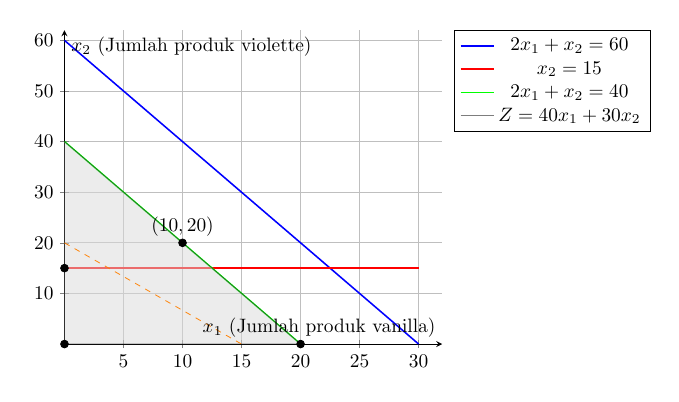
\begin{tikzpicture}[scale=0.7]
    \begin{axis}[
        axis lines=middle,
        grid=both,
        xmin=0, xmax=32,
        ymin=0, ymax=62,
        xtick={0,5,...,30},
        ytick={0,10,...,60},
        xlabel={$x_1$ (Jumlah produk vanilla)},
        ylabel={$x_2$ (Jumlah produk violette)},
        legend pos=outer north east
    ]
    
    % Kendala bahan baku A: 2x₁ + x₂ ≤ 60
    \addplot[domain=0:30, thick, blue] {60-2*x};
    \addlegendentry{$2x_1 + x_2 = 60$}
    
    % Kendala bahan baku B: 2x₂ ≤ 30
    \addplot[domain=0:30, thick, red, samples=2] {15};
    \addlegendentry{$x_2 = 15$}
    
    % Kendala tenaga kerja: 2x₁ + x₂ ≤ 40
    \addplot[domain=0:20, thick, green] {40-2*x};
    \addlegendentry{$2x_1 + x_2 = 40$}
    
    % Daerah fisibel
    \addplot[fill=gray!30, opacity=0.5] coordinates {
        (0,0) (0,15) (0,40) (10,20) (20,0) (0,0)
    } \closedcycle;
    
    % Titik-titik sudut
    \addplot[mark=*, color=black] coordinates {(0,0)} node[anchor=north east] {$(0,0)$};
    \addplot[mark=*, color=black] coordinates {(0,15)} node[anchor=east] {$(0,15)$};
    \addplot[mark=*, color=black] coordinates {(10,20)} node[anchor=south] {$(10,20)$};
    \addplot[mark=*, color=black] coordinates {(20,0)} node[anchor=north west] {$(20,0)$};
    
    % Garis fungsi tujuan
    \addplot[domain=0:30, dashed, orange] {(600-40*x)/30};
    \addlegendentry{$Z = 40x_1 + 30x_2$}
    
    \end{axis}
    \end{tikzpicture}
    \caption{Daerah Fisibel dan Titik Optimal - Masalah Produksi PT Yummy Food}
    \end{figure}
    
    Langkah 5: Menentukan titik-titik sudut daerah fisibel:
    \begin{align*}
    &(0,0) && \text{titik asal} \\
    &(0,15) && \text{titik potong kendala bahan baku B dengan sumbu } x_2 \\
    &(10,20) && \text{titik potong kendala bahan baku B dan kendala tenaga kerja} \\
    &(20,0) && \text{titik potong kendala tenaga kerja dengan sumbu } x_1
    \end{align*}
    
    Titik $(10,20)$ diperoleh dari penyelesaian sistem persamaan:
    \begin{align*}
    x_2 &= 15 \quad \ldots (1) \\
    2x_1 + 1x_2 &= 40 \quad \ldots (2)
    \end{align*}
    
    Substitusi persamaan (1) ke persamaan (2):
    \begin{align*}
    2x_1 + 15 &= 40 \\
    2x_1 &= 25 \\
    x_1 &= 12.5
    \end{align*}
    
    Jadi titik potongnya seharusnya adalah $(12.5,15)$.
    
    Titik $(10,20)$ diperoleh dari penyelesaian sistem persamaan:
    \begin{align*}
    2x_1 + 1x_2 &= 40 \quad \ldots (1) \\
    2x_1 + 1x_2 &= 60 \quad \ldots (2)
    \end{align*}
    
    Karena kedua persamaan memiliki koefisien sama, maka tidak ada titik potong unik. Berarti ada kesalahan dalam penentuan titik sudut ini.
    
    Mari koreksi:
    
    Titik sudut yang benar adalah:
    \begin{align*}
    &(0,0) && \text{titik asal} \\
    &(0,15) && \text{titik potong kendala bahan baku B dengan sumbu } x_2 \\
    &(12.5,15) && \text{titik potong kendala bahan baku B dan kendala tenaga kerja} \\
    &(20,0) && \text{titik potong kendala tenaga kerja dengan sumbu } x_1
    \end{align*}
    
    Langkah 6: Mengevaluasi fungsi tujuan di setiap titik sudut:
    \begin{align*}
    Z(0,0) &= 40(0) + 30(0) = 0 \\
    Z(0,15) &= 40(0) + 30(15) = 450 \\
    Z(12.5,15) &= 40(12.5) + 30(15) = 500 + 450 = 950 \\
    Z(20,0) &= 40(20) + 30(0) = 800
    \end{align*}
    
    Nilai maksimum fungsi tujuan secara matematis tercapai pada titik
    $(12.5,15)$ dengan nilai $Z = 950$ Namun karena secara fisik tidak dapat
    membuat produksi sebanyak 0.5 barang, maka dibulatkan menjadi $(12,15)$
    
    \textbf{Pemecahan Bilangan Bulat:}
    
    Karena produk harus diproduksi dalam jumlah bulat (tidak mungkin
    memproduksi 0,5 barang), maka kita perlu mencari solusi bilangan bulat.
    Kandidat titik bilangan bulat di sekitar $(12.5,15)$ yang mana menghasilkan
    nilai maksimum $Z = 930$;
    \begin{figure}[H]
    \centering
    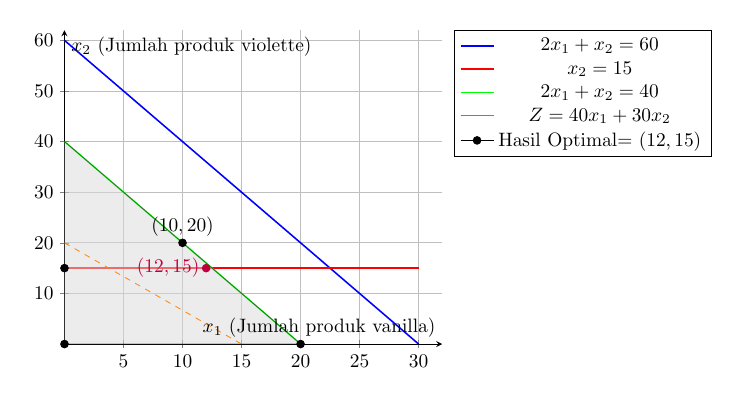
\begin{tikzpicture}[scale=0.7]
    \begin{axis}[
        axis lines=middle,
        grid=both,
        xmin=0, xmax=32,
        ymin=0, ymax=62,
        xtick={0,5,...,30},
        ytick={0,10,...,60},
        xlabel={$x_1$ (Jumlah produk vanilla)},
        ylabel={$x_2$ (Jumlah produk violette)},
        legend pos=outer north east
    ]
    
    % Kendala bahan baku A: 2x₁ + x₂ ≤ 60
    \addplot[domain=0:30, thick, blue] {60-2*x};
    \addlegendentry{$2x_1 + x_2 = 60$}
    
    % Kendala bahan baku B: 2x₂ ≤ 30
    \addplot[domain=0:30, thick, red, samples=2] {15};
    \addlegendentry{$x_2 = 15$}
    
    % Kendala tenaga kerja: 2x₁ + x₂ ≤ 40
    \addplot[domain=0:20, thick, green] {40-2*x};
    \addlegendentry{$2x_1 + x_2 = 40$}
    
    % Daerah fisibel
    \addplot[fill=gray!30, opacity=0.5] coordinates {
        (0,0) (0,15) (0,40) (10,20) (20,0) (0,0)
    } \closedcycle;
    
    % Titik-titik sudut
    \addplot[mark=*, color=black] coordinates {(0,0)} node[anchor=north east] {$(0,0)$};
    \addplot[mark=*, color=black] coordinates {(0,15)} node[anchor=east] {$(0,15)$};
    \addplot[mark=*, color=black] coordinates {(10,20)} node[anchor=south] {$(10,20)$};
    \addplot[mark=*, color=black] coordinates {(20,0)} node[anchor=north west] {$(20,0)$};
    \addplot[mark=*, color=purple] coordinates {(12,15)} node[anchor=east] {$(12,15)$};
    
    % Garis fungsi tujuan
    \addplot[domain=0:30, dashed, orange] {(600-40*x)/30};
    \addlegendentry{$Z = 40x_1 + 30x_2$}

    \addlegendentry{Hasil Optimal= $(12,15)$}
    
    \end{axis}
    \end{tikzpicture}
    \caption{Grafik hasil Optimal - Masalah Produksi PT Yummy Food}
    \end{figure}
\end{enumerate}

\end{document}
